\chapter{Experimental Apparatus}
\label{CHAPTER:ExperimentalApparatus}

% \glsresetall % Resetting all acronyms

%%%%%%%%%%%%%%%%%%%%%%%%%%%%%%%%%%%%%%%%%%%%%%%%%%%%%%%%%%%%%%%%%%%%%%%%%%%%%%%%%%%%%%%
%%% SECTION
%%%%%%%%%%%%%%%%%%%%%%%%%%%%%%%%%%%%%%%%%%%%%%%%%%%%%%%%%%%%%%%%%%%%%%%%%%%%%%%%%%%%%%%
\section{The Large Hadron Collider}
\label{SECTION:ExperimentalApparatus_LHC}

% Status: DONE (reviewed D. Colling x1)

% CERN and LHC Location
The \gls{LHC}~\cite{ARTICLE:LHCDesignReportVol1,ARTICLE:LHCMachine} is currently the world's largest particle accelerator and is capable of producing the highest energy particle beams ever made by mankind. This machine has total perimeter of $26.7\,\kilo\meter$ and was built at the \gls{CERN} in a circular tunnel, which previously housed the \gls{LEP} collider~\cite{LEPTDR:LEPInjectorStudyGroup}, at an average depth of $100\,\meter$ below ground under the Franco-Swiss border near Geneva, Switzerland. A diagram of the \gls{LHC} tunnel and its experiments can be found at figure \ref{FIGURE:ExperimentalApparatus_LHCLayoutUnderground}.

\begin{figure}[!htb]
  \centering
  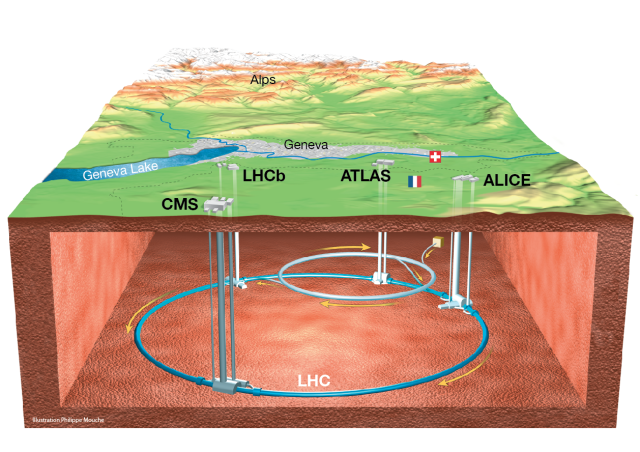
\includegraphics[width=0.70\textwidth]{Chapter02/LHC/Images/LHCUnderGroundDiagram.png}
  \caption{Underground diagram of the Geneva area showing the \gls{LHC} and its experiments location~\cite{IMAGEREF:LHCDiagram}.}
  \label{FIGURE:ExperimentalApparatus_LHCLayoutUnderground}
\end{figure}

% Structure and experiments
The \gls{LHC} is a synchrotron machine with the capability of accelerating two particle beams in opposite directions in two separate beam pipes. These beams only cross and are forced to collide in four points of the accelerator where particle detectors are installed to observe the products of such collisions. This experiments are: \gls{ATLAS}~\cite{ARTICLE:TheATLASExperiment}, \gls{CMS}~\cite{ARTICLE:TheCMSExperiment}, \gls{LHCb}~\cite{ARTICLE:TheLHCbExperiment} and \gls{ALICE}~\cite{ARTICLE:TheALICEExperiment}.
% Add other experiments?

% Objective
The objective of the \gls{LHC} program is to investigate physics at the $\TeV$ scale, more specifically to understand the electroweak symmetry breaking and if this phenomenon could be explained by the Higgs mechanism. There are many \gls{BSM} theories that predict new physics at this energy regime, making the \gls{LHC} the perfect machine to investigate such phenomena. \gls{ATLAS} and \gls{CMS} are general-purpose detectors which aim to investigate a broad spectrum of physics. The \gls{LHCb} detector is used to study processes that involve the decay of b-flavoured hadrons. The \gls{ALICE} detector is optimised to look at heavy-ion collisions and to investigate the properties of the extreme density medium that is formed.

% CERN accelerator chain
The \gls{LHC} is only the last element of a complex accelerator chain which step-by-step increases the energy of the particles that will eventually be collided~\cite{ARTICLE:LHCMachine}. Protons are initially obtained by stripping the electrons of hydrogen gas. This process happens at the begging of the \gls{LINAC2} which then accelerates them up to the energy of $50\,\MeV$. After this initial step, protons are injected into the \gls{PSB} and the energy ramps ups to $1.4\,\GeV$. Particles are then passed to the \gls{PS} where the energy further increases to $25\,\GeV$. Subsequently they are injected into the \gls{SPS} where the particle energy reaches $450\,\GeV$. Finally, protons pass to the \gls{LHC} where they can be accelerated to a maximum energy of $7\,\TeV$. A simplified diagram of the \gls{CERN} accelerator chain can be found in figure \ref{FIGURE:ExperimentalApparatus_LHCAccelaratorChain}. 
Normal operation of the \gls{LHC} therefore depends on all the upstream accelerators availability. The turn around time, the time necessary to stop the accelerator from running and restart collisions, can be as low as 2 hours. When stable beams are achieved, a single proton fill can be used to collide protons for up to 24 hours, but it is common to restart more frequently to profit from the higher collision rates possible right at the beginning of a new fill.

\begin{figure}[!htb]
  \centering
  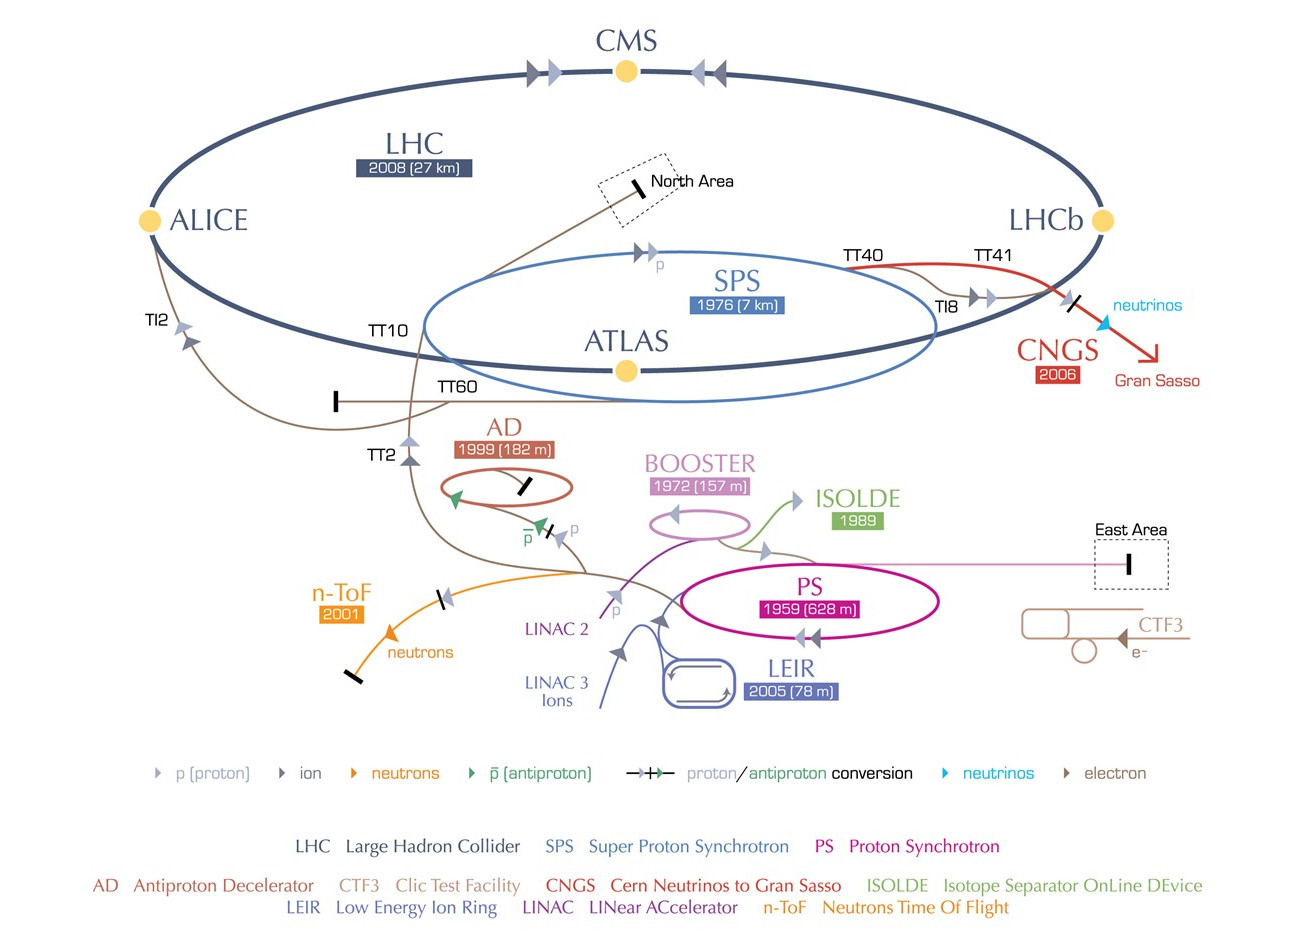
\includegraphics[width=0.90\textwidth]{Chapter02/LHC/Images/CERNAcceleratorComplex.jpg}
  \caption{Diagram of the \gls{CERN} accelerator complex~\cite{IMAGEREF:CERNAcceleratorComplex}.}
  \label{FIGURE:ExperimentalApparatus_LHCAccelaratorChain}
\end{figure}

% LHC modes of opperation
Each beam pipe can be filled with proton or heavy ions. Three modes of operation have been tried: proton-proton, proton-lead ion and lead ion-lead ion. By changing the incoming particles we are changing the quantity of nucleons present at each interaction. The maximum design energy per proton is $7\,\TeV$ and is $2.76\,\TeV$ for each lead nucleon. The maximum design luminosity for proton-proton collisions is $10^{34}\,\cm^{-2}\second^{-1}$ and $10^{27}\,\cm^{-2}\second^{-1}$ for lead ion-lead ion collisions.

% LHC structure
Particle beams trajectories are curved by 1232 niobium-titanium superconducting dipole magnets each with a length of $14.3\,\meter$. They are cooled with superfluid helium to $1.9\,\kelvin$ and produce the necessary magnetic field of $8.4\,\tesla$. Eight \gls{RF} cavities located at the \gls{LHC} point 4 are used to accelerate the beams. At nominal operation the \gls{LHC} will steer 2808 bunches composed up to $10^{11}$ protons separated by $25\,\ns$ in each direction. Some of the key parameters of the \gls{LHC} proton-proton and lead-lead operation can be found in table \ref{TABLE:ExperimentalApparatus_LHCMachineParameters}.

\begin{table}[!htb]
  \centering
  \begin{threeparttable}
    \begin{tabular}{|lcccc|}
    \hline 
                                  &              &           \textit{pp} &         \textbf{HI} &  \\
    \hline\hline
    Energy per nucleon            & E            &                     7 &                2.76 &                 $\TeV$ \\
    Dipole field at 7 TeV         & \textit{B}   &                  8.33 &                8.33 &               $\tesla$ \\
    Design Luminosity\tnote{*}    & $\mathcal{L}$ &            $10^{34}$ &           $10^{27}$ & $\cm^{-2}\second^{-1}$ \\
    Bunch separation              &              &                    25 &                 100 &                  $\ns$ \\
    No. of bunches                & $k_B$        &                  2808 &                 592 &                        \\
    No. particles per bunch       & $N_p$        & $1.15 \times 10^{11}$ & $7.0 \times 10^{7}$ &                        \\
    \hline
    \hline
    \textbf{Collisions}           &              &  &  &  \\
    \hline
    $\beta$-value at IP           & $\beta^{*}$  &                  0.55 &                 0.5 &        $\meter$ \\
    RMS beam radius at IP         & $\sigma^{*}$ &                  16.7 &                15.9 &  $\micro\meter$ \\
    Luminosity lifetime           & $\tau_L$     &                    15 &                   6 &         $\hour$ \\
    Number of collisions/crossing & $n_c$        &          $\approx 20$ &                   - &                 \\
    \hline
    \end{tabular}
    \begin{tablenotes}
      \item[*] For heavy-ion (HI) operation the design luminosity for Pb-Pb collisions is given.
    \end{tablenotes}
  \end{threeparttable}
  \caption[LHC parameters relevant for detectors]{The machine parameters relevant for the 
                                                  LHC detectors.\cite{CMSTDR:CMSPhysicsVol1}}
  \label{TABLE:ExperimentalApparatus_LHCMachineParameters}
\end{table}


At the \gls{LHC} we are looking for extremely rare processes. As it can be seen in figure \ref{FIGURE:ExperimentalApparatus_LHCCrossSections}, the production cross section of a \gls{SM} Higgs boson is more than 9 orders of magnitude smaller than the total proton-proton cross section. 

\begin{figure}[!htb]
  \centering
  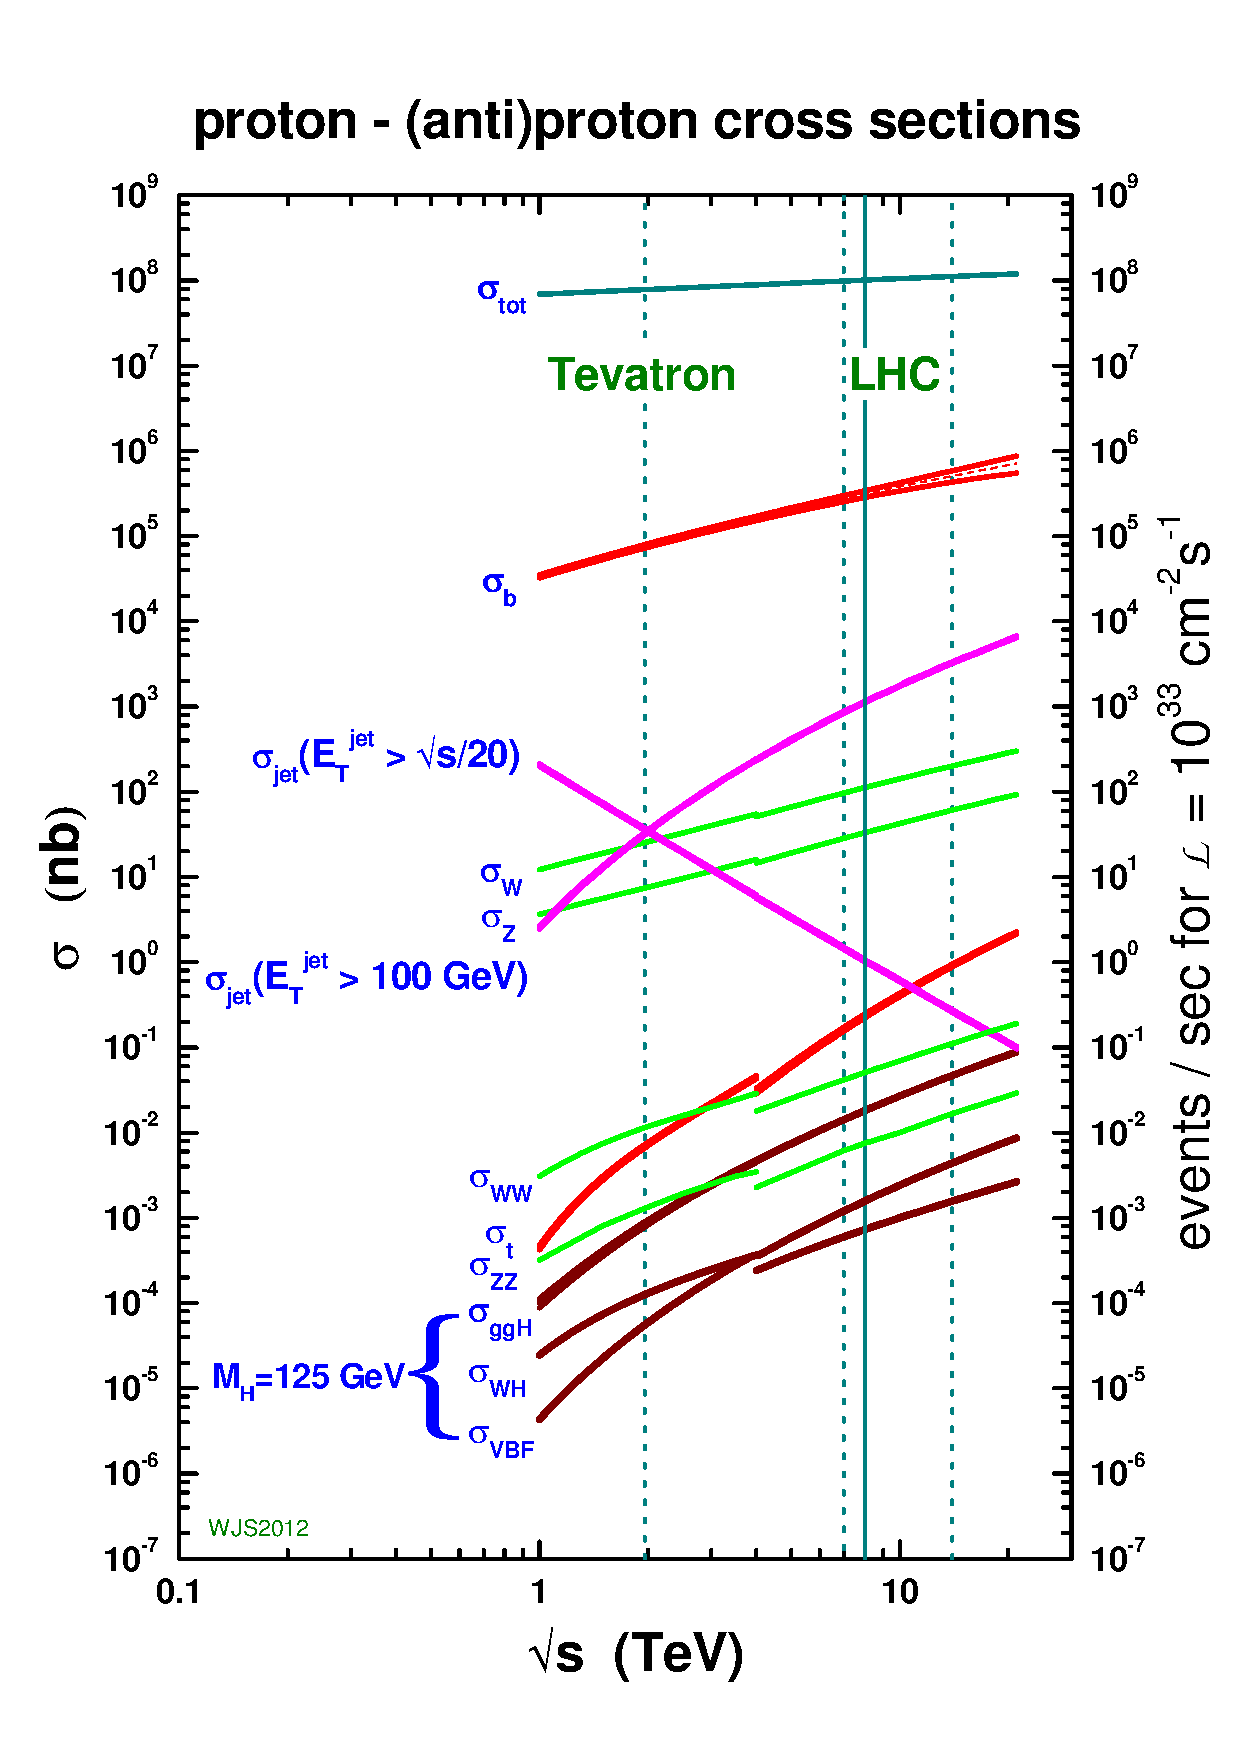
\includegraphics[width=0.50\textwidth]{Chapter02/LHC/Images/crosssections2012_v5}
  \caption{Cross sections for several processes for collisions of antiproton-proton and proton-proton as a function of the center of mass energy~\cite{ARTICLE:TheCMSExperiment}.}
  \label{FIGURE:ExperimentalApparatus_LHCCrossSections}
\end{figure}

To be able to record and study such rare processes we need to produce a significant number of collisions. For this purpose the \gls{LHC} was designed to operate at high instantaneous luminosity, L. This quantity is defined as,

\begin{equation}
L=\frac{N_{b}^{2}n_{b}f_{\text{rev}}\gamma}{4\pi\epsilon_{n}\beta^{*}}F,
\end{equation}

where $N_{b}$ is the number of protons per bunch, $n_{b}$ is the number of bunches, $f_{\text{rev}}$ is the frequency of revolution, $\gamma$ is the Lorentz factor, $\epsilon_{n}$ is the normalized emittance, $\beta^{*}$ is the beta function at the collision point and $F$ is the reduction factor due to the crossing angle.

%%%%%%%%%%%%%%%%%%%%%%%%%%%%%%%%%%%%%%%%%%%%%%%%%%%%%%%%%%%%%%%%%%%%%%%%%%%%%%%%%%%%%%%
%%% SUBSECTION
%%%%%%%%%%%%%%%%%%%%%%%%%%%%%%%%%%%%%%%%%%%%%%%%%%%%%%%%%%%%%%%%%%%%%%%%%%%%%%%%%%%%%%%
\subsection{Running and performance}
\label{SUBSECTION:ExperimentalApparatus_CMS_RunningAndPerformance}

%Status: Done (reviewed D. Colling x1)

%Historical
Operation of the \gls{LHC} started when the first beams circulated in the machine in September 2008. Unfortunately, only a few days later, a faulty weld between two dipole magnets caused a significant magnet quench which in turn damaged several dipoles and a simultaneous leak of a significant amount of helium happened. The event showed that beyond the repair of the affected systems the accelerator needed a significant consolidation program to allow it to return to activity~\cite{ARTICLE:CMSReportIncident19Sep2008}. This consolidation program took over one year to finalise and to prevent further possible problems and allow better understanding of the machine while maximizing physics reach, it was decided to initially run the \gls{LHC} at $7\,\TeV$ center-of-mass energy.
First collisions happened at November 2009 just at the \gls{SPS} injection energy of $450\,\GeV$ giving start to the \gls{LHC} run I.

The collision energy was finally ramped up to $7\,\TeV$ with first collisions being observed during March 2010. Operation at this energy continued until the end of 2011, with a peak luminosity being achieved of $3.7 \times 10^{33} \centi\meter^{-2}\second^{-1}$. The total integrated luminosity delivered to \gls{CMS} was $6.1\,\femto\barn^{-1}$ with the total actually recorded being $5.6\,\femto\barn^{-1}$. During 2012 with the increased knowledge of the accelerator it was possible to increase the centre-of-mass energy further to $8\,\TeV$, eventually reaching peak luminosity of $7.7 \times 10^{33}\,\centi\meter^{-2}\second^{-2}$ and delivering integrated luminosity of $23.3\,\femto\barn^{-1}$ to \gls{CMS} of which $21.79\,\femto\barn^{-1}$ were recorded. Figure \ref{FIGURE:ExperimentalApparatus_CMS_IntegratedLumi_pp_2010-2012} shows the delivered luminosity in the period 2010-2013 over time.

\begin{figure}[!htb]
  \centering
  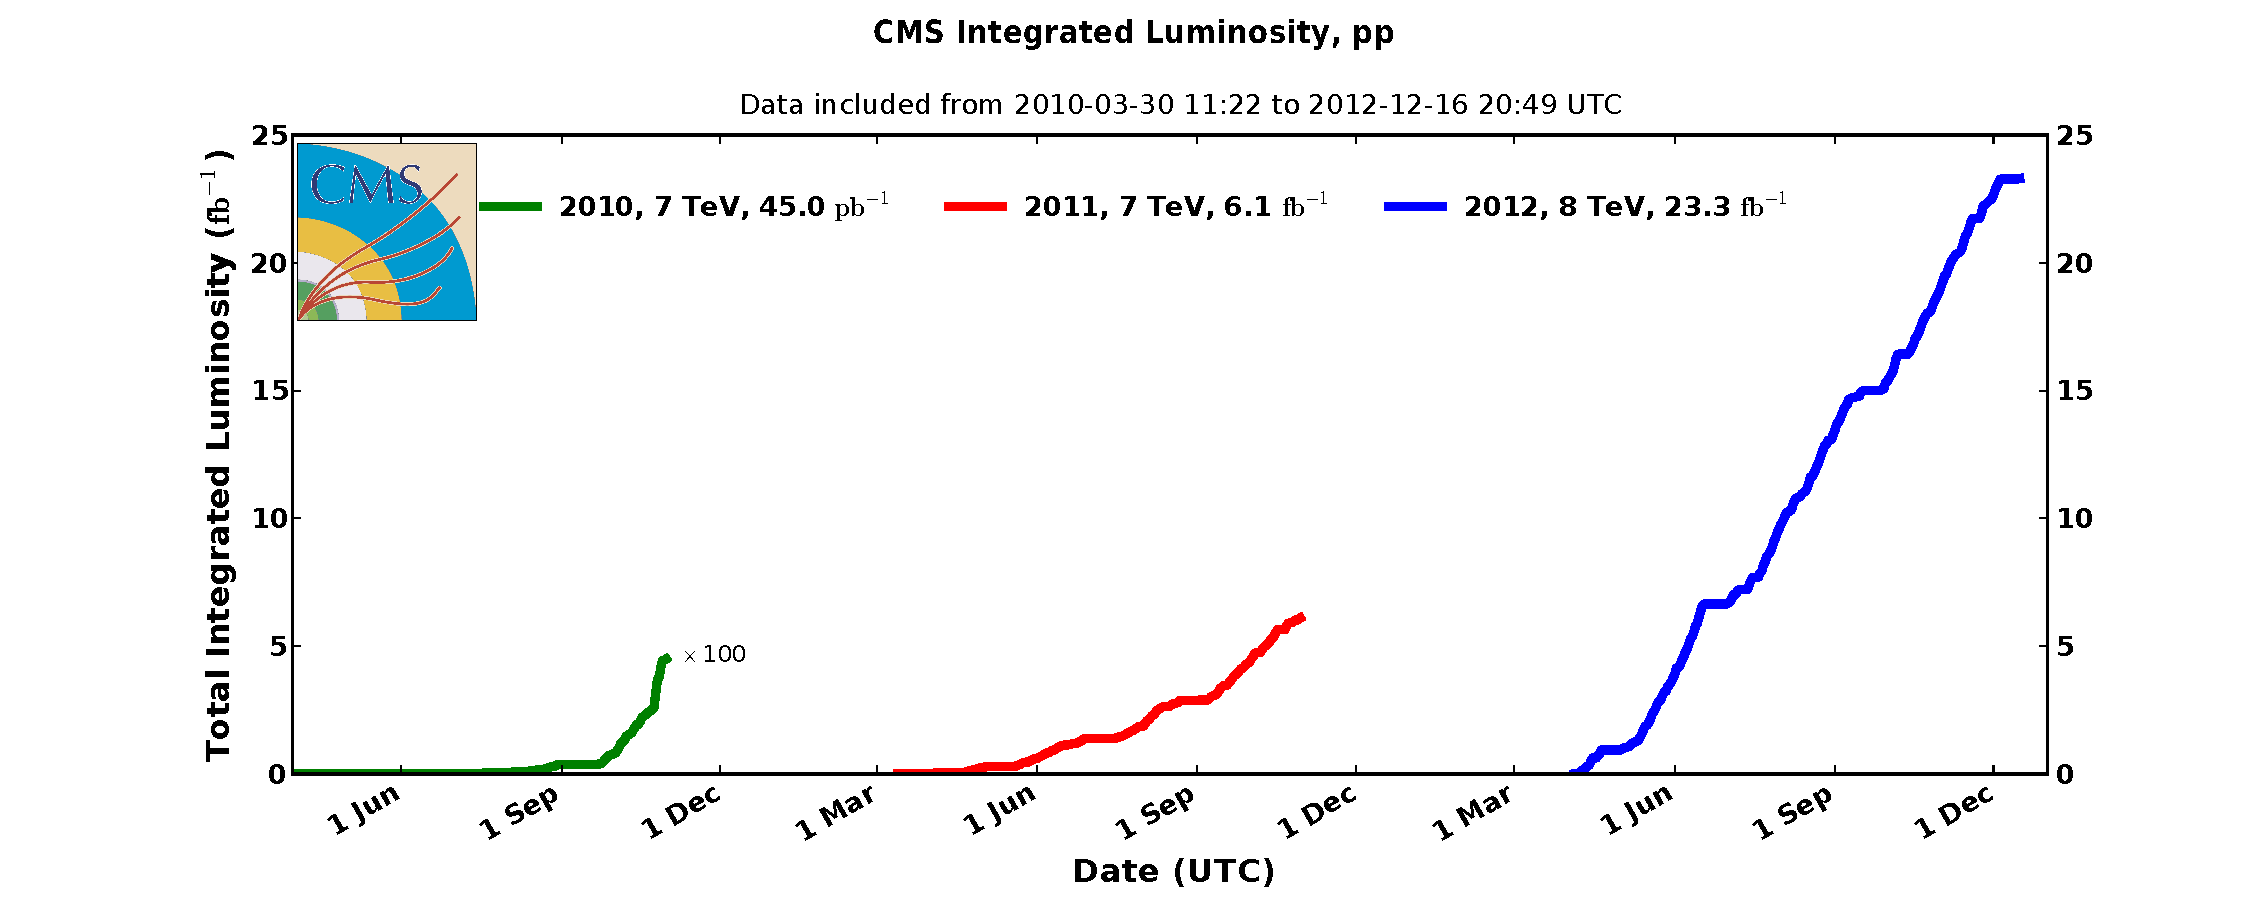
\includegraphics[width=1.00\textwidth]{Chapter02/CMS/Images/CMS_IntegratedLumi_pp_2010-2012}
  \caption{Cumulative luminosity versus day delivered to CMS during stable beams and for p-p collisions. This is shown for 2010 (green), 2011 (red) and 2012 (blue) data-taking~\cite{IMAGEREF:CMSIntegratedLuminosity}.}
  \label{FIGURE:ExperimentalApparatus_CMS_IntegratedLumi_pp_2010-2012}
\end{figure}

For physics usage, data needs to undergo a certification process. In this process specialists from each \gls{CMS} subsystem check that no problem has happened during data taking that would bias or invalidate the recorded events. For 2011 a total of $5.1\,\femto\barn^{-1}$ and for 2012 a total $19.7\,\femto\barn^{-1}$ were considered of good quality for physics. 

In order to achieve high integrated luminosity \gls{LHC} collides particle bunches up to 40 million times a second, and many interactions may happen simultaneously, this effect is called \gls{PU}. Figure \ref{FIGURE:ExperimentalApparatus_CMS_PileIp_pp_2012} shows the distribution of the mean number of interaction per bunch crossing during 2012 at the \gls{CMS} experiment.

\begin{figure}[!htb]
  \centering
  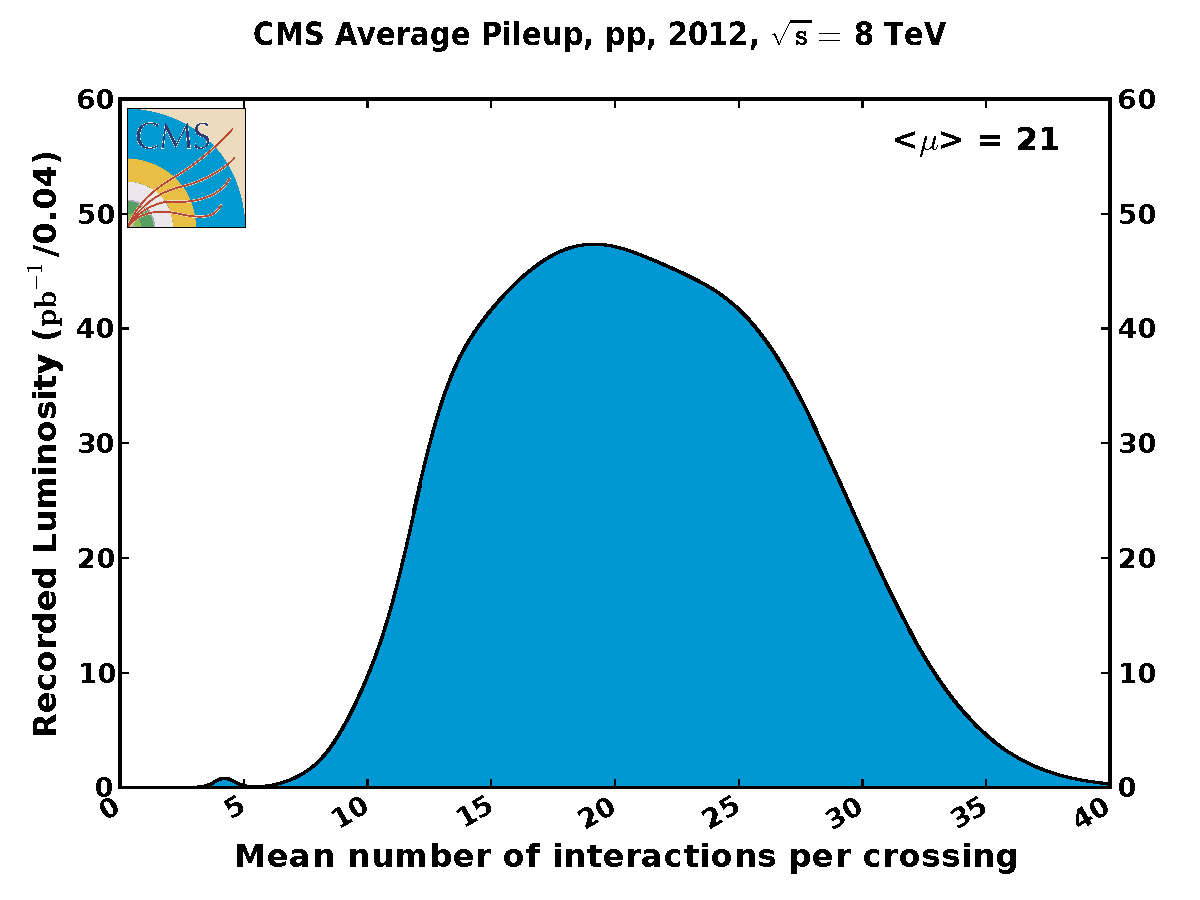
\includegraphics[width=0.60\textwidth]{Chapter02/CMS/Images/CMS_PileIp_pp_2012}
  \caption{Mean number of interactions per bunch crossing at the CMS experiment during 2012. The year's total mean number of interactions per crossing, $<\mu>$, was of 21 collisions~\cite{IMAGEREF:CMSAveragePileUp2012}.}
  \label{FIGURE:ExperimentalApparatus_CMS_PileIp_pp_2012}
\end{figure}

%%%%%%%%%%%%%%%%%%%%%%%%%%%%%%%%%%%%%%%%%%%%%%%%%%%%%%%%%%%%%%%%%%%%%%%%%%%%%%%%%%%%%%%
%%% SECTION
%%%%%%%%%%%%%%%%%%%%%%%%%%%%%%%%%%%%%%%%%%%%%%%%%%%%%%%%%%%%%%%%%%%%%%%%%%%%%%%%%%%%%%%
\section{The Compact Muon Solenoid Experiment}
\label{SECTION:ExperimentalApparatus_CMS}

%Status: Done (reviewed D. Colling x1)

The \acrfull{CMS} experiment~\cite{ARTICLE:TheCMSExperiment} is a general purpose experiment located at the \gls{LHC} point 5, near the village of Cessy, France. It was designed to be a high performance detector studying collisions at its centre. It is composed of several subsystems in a classic onion shaped structure. A diagram of the experiment can be found in figure \ref{FIGURE:ExperimentalApparatus_CMS_Layout_Diagram}.

\begin{figure}[!htb]
  \centering
  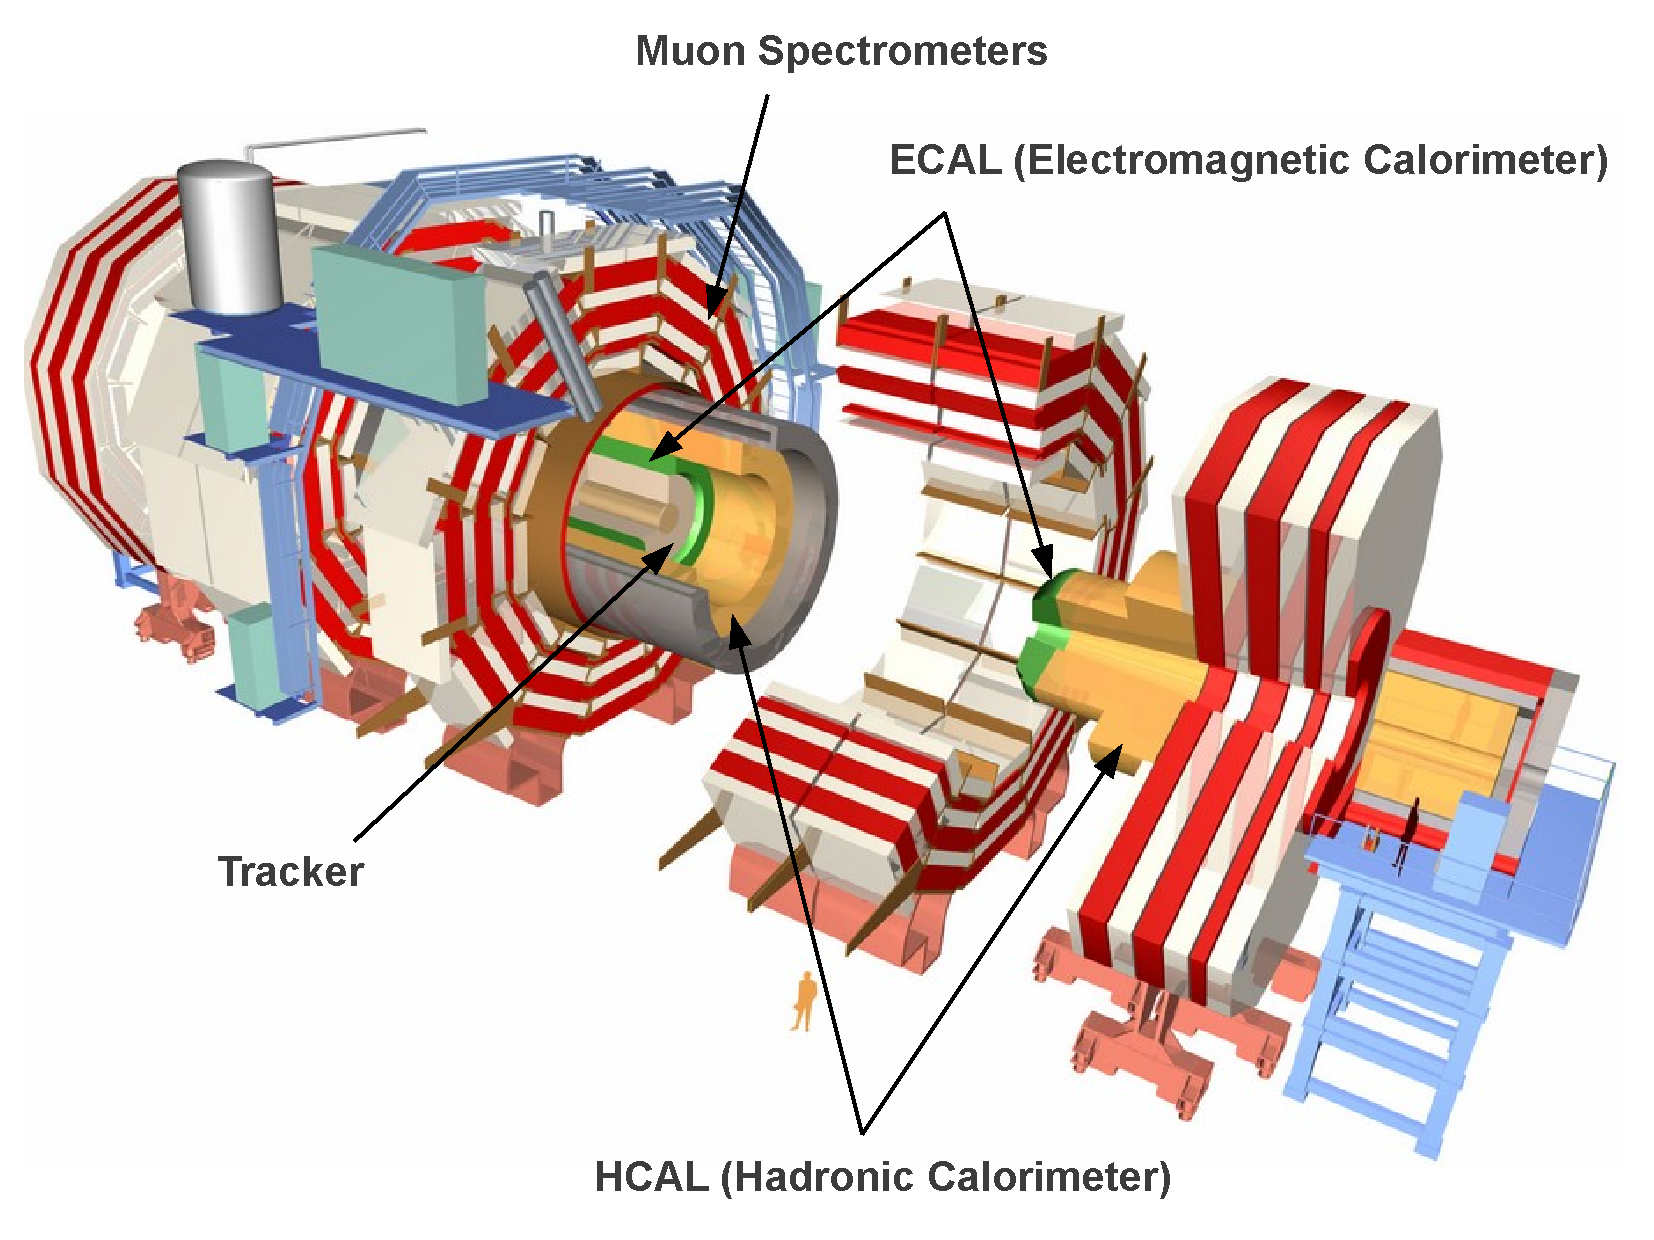
\includegraphics[width=1.00\textwidth]{Chapter02/CMS/Images/CMS_Layout_Diagram.pdf}
  \caption{Diagram of \gls{CMS} experiment showing the experiment in an open configuration and highlighting the position of its sub-detectors~\cite{IMAGEREF:CERNPublic_CMSDiagram}.}
  \label{FIGURE:ExperimentalApparatus_CMS_Layout_Diagram}
\end{figure}

The main driving motivation for its design was to investigate the electroweak symmetry breaking and the Higgs mechanism which at the design time was presumed to be the most likely explanation. Many alternative theories to the standard model predict new particles which could be observed at the $\TeV$ scale. \gls{CMS} as a multi-purpose experiment is well suited to search for these new scenarios. If found, such new physics may allow us to understand some of the currently open questions in particle physics, like providing particle candidates for dark matter. Furthermore, some of these possible new physics signals could point the way towards a grand unified theory. \gls{CMS} is also capable of operating while the \gls{LHC} is colliding heavy ions and has a rich program covering the study of matter at extreme temperatures, densities and parton momentum fraction (low-x).

The requirements imposed on the \gls{CMS} design to meet its physics goals can be summarized in the following table~\cite{ARTICLE:CMSTechnicalProposal,ARTICLE:TheCMSExperiment}:

\begin{itemize}
  \item Good muon identification and momentum resolution over a wide range of momenta and angles, good dimuon mass resolution ($\approx 1\%$ at $100\,GeV$), and the ability to determine unambiguously the charge of muons with $\pt<1\,\TeV$.
  \item Good charged-particle momentum resolution and reconstruction efficiency in the inner tracker. Efficient triggering and offline tagging of $\tau$'s and b-jets, requiring pixel detectors close to the interaction region.
  \item Good electromagnetic energy resolution, good diphoton and dielectron mass resolution ($\approx 1\%$ at $100\,\GeV$), wide geometric coverage, $\pi^0$ rejection, and efficient photon and lepton isolation at high luminosities.
  \item Good missing-transverse-energy and dijet-mass resolution, requiring hadron calorimeters with a large hermetic geometric coverage and with fine lateral segmentation.
\end{itemize}

The final detector design fulfils all these requirements. The experiment is compact compared to the other \gls{LHC} experiments being $22\,\meter$ long and $15\,\meter$ in diameter. Although small, it is the heaviest of the four big detectors at 12500 tonnes. Its high density is a direct consequence of it producing the highest magnetic field at $4\,\tesla$ and therefore needing more material for it to be contained in its return yoke. 

%%%%%%%%%%%%%%%%%%%%%%%%%%%%%%%%%%%%%%%%%%%%%%%%%%%%%%%%%%%%%%%%%%%%%%%%%%%%%%%%%%%%%%%
%%% SUBSECTION
%%%%%%%%%%%%%%%%%%%%%%%%%%%%%%%%%%%%%%%%%%%%%%%%%%%%%%%%%%%%%%%%%%%%%%%%%%%%%%%%%%%%
\subsection{Geometry and conventions}
\label{SECTION:ExperimentalApparatus_CMS_GeometryConventions}

% STATUS: DONE (reviewed D. Colling x1)

The adopted coordinate system has it origin in the center of \gls{CMS}, where the nominal collision point is located, the \textit{y}-axis points vertically upwards, and the \textit{x}-axis points radially inward in the direction of the centre of the \gls{LHC}. The \text{z}-axis points along the beam line towards the Jura mountains from the \gls{LHC} point 5. The azimuthal angle $\phi$ is measured from the \textit{x}-axis in the \textit{x-y} plane. The polar angle $\theta$ is measured from the \textit{z}-axis.

We define pseudorapidity as $\eta = -ln(tan(\theta/2))$. All transverse quantities, like the transverse momentum ($p_\perp$), are measured in the transverse plane to the beam axis. The imbalance of energy is also measured in the \textit{x-y} plane and is denoted as $E^{miss}_\perp$.

%%%%%%%%%%%%%%%%%%%%%%%%%%%%%%%%%%%%%%%%%%%%%%%%%%%%%%%%%%%%%%%%%%%%%%%%%%%%%%%%%%%%%%%
%%% SUBSECTION
%%%%%%%%%%%%%%%%%%%%%%%%%%%%%%%%%%%%%%%%%%%%%%%%%%%%%%%%%%%%%%%%%%%%%%%%%%%%%%%%%%%%
\subsection{Inner tracking system}
\label{SUBSECTION:ExperimentalApparatus_CMS_Tracker}

% STATUS: DONE (reviwed J.Pela x1) (reviewed D. Colling x1)

The inner tracking system is the closest detector to the beam axis and the interaction region~\cite{CMSTDR:CMSTracker,CMSTDR:CMSTrackerAddendum}. Its function is to measure the trajectory of all charged particles with momentum above 1 $\GeV$ being produced at each \gls{LHC} collision. With the help of the strong magnetic field produced by the \gls{CMS} magnet, particle trajectories are bent allowing for charge and momentum determination. With the resulting tracks it is then possible to determine the primary vertex as well as secondary vertices like other lower energy proton-proton collisions or displaced vertices from the decay of long-lived particles like B-hadrons.

Building a tracking system for an experiment at the \gls{LHC} is very challenging. Such system at design luminosity will be hit by an average of 1000 particles per beam crossing at a rate approaching $40\,\mega\hertz$. It needs to be a fast, efficient, high granularity detector, radiation hard and as thin as possible to not deflect the incoming particles trajectory. At each layer the occupancy should be of the order of $1\%$ or lower. These design requirements have led to a tracker design entirely based on silicon detector technology. 

The volume near the interaction point can be split according to the charged particle flux into three regions:

\begin{itemize}
  \item $r<10\,\centi\meter$: highest particle flux, up to $\approx 10^8 \centi\meter^{-2}\second^{-1}$ at $r \approx 4 \centi\meter$, pixel detectors are used. The pixel size is $\approx 100 \times 150\,\micro\meter^2$, which translates into an occupancy of $10^{-4}$ per \gls{LHC} bunch crossing.
  \item $20<r<55\,\centi\meter$: particle flux decreases enough to use silicon micro-strips with a minimum cell size of $10\,\centi\meter \times 80\,\micro\meter$, leading to an occupancy of $\approx 2-3\%$ per \gls{LHC} bunch crossing.
  \item $50<r<110\,\centi\meter$: most outer region of the tracker, particle flux is low enough to use larger pitch silicon micro-strips. The maximum cell size is of $25\,\centi\meter$ $\times 180\,\micro\meter$, and occupancy is of the order of $\approx 1\%$.
\end{itemize}

The \gls{CMS} tracker final configuration is composed of a pixel detector with three barrel layers at radii between $4.4\,\centi\meter$ and $10.2\,\centi\meter$ and 2 disks on each side of the barrel. A silicon strip tracker with 10 barrel detection layers extending up to $1.1\,\meter$ with 3 inner tracker plus 9 endcap disks on each side of the barrel. A schematic of this detector module distribution can be found at figure \ref{FIGURE:ExperimentalApparatus_CMS_Tracker_Layout}. This detector has an acceptance covering up to pseudorapidity of $|\eta|<2.5$ and has a total active area of about $200\,\meter^2$ making it the largest silicon tracker ever built. 

\begin{figure}[!htb]
  \centering
  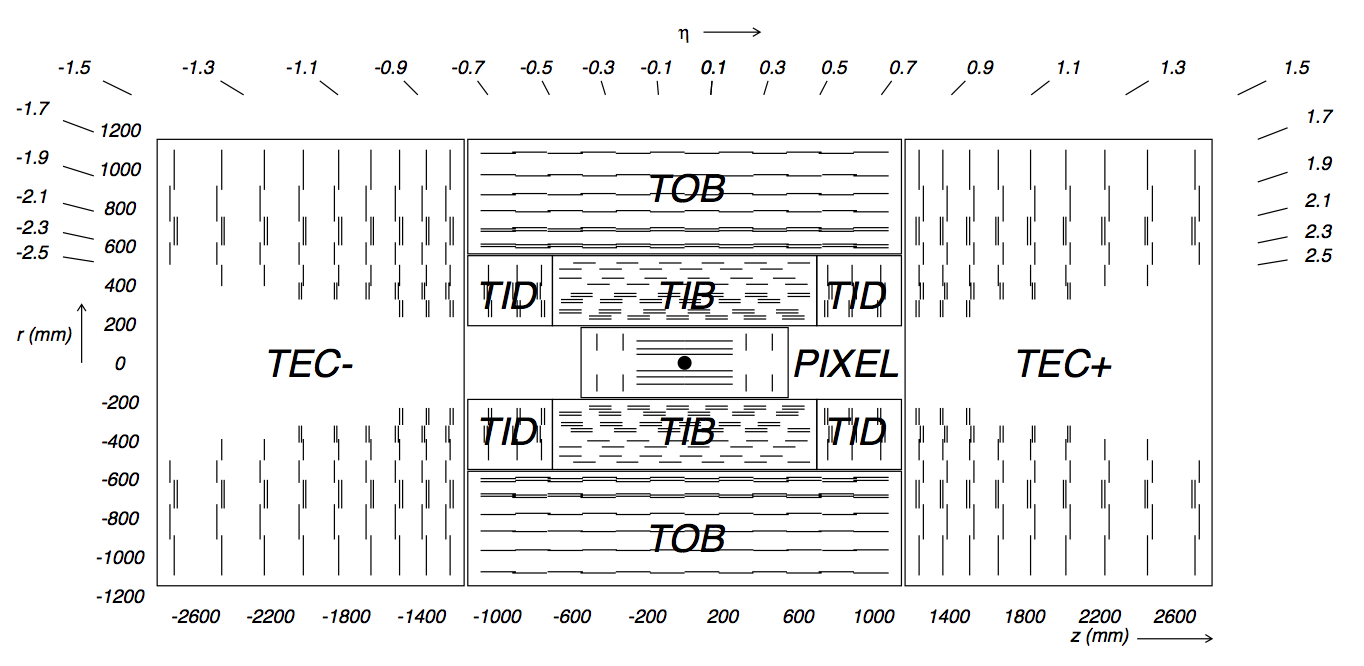
\includegraphics[width=1.0\textwidth]{Chapter02/CMS/Images/CMS_Tracker_Layout.png}
  \caption{Schematic cross section of the CMS tracker~\cite{ARTICLE:TheCMSExperiment}. Each line represents a detector module. Double lines represent dual surface back-to-back detector modules. The inner tracker components are shown components: \gls{TEC}, \gls{TOB}, \gls{TID}, \gls{TIB} and Pixels. }
  \label{FIGURE:ExperimentalApparatus_CMS_Tracker_Layout}
\end{figure}

%%%%%%%%%%%%%%%%%%%%%%%%%%%%%%%%%%%%%%%%%%%%%%%%%%%%%%%%%%%%%%%%%%%%%%%%%%%%%%%%%%%%%%%
%%% SUBSECTION
%%%%%%%%%%%%%%%%%%%%%%%%%%%%%%%%%%%%%%%%%%%%%%%%%%%%%%%%%%%%%%%%%%%%%%%%%%%%%%%%%%%%
\subsection{Electromagnetic Calorimeter}
\label{SUBSECTION:ExperimentalApparatus_CMS_ECAL}

% Status: DONE (reviewed D. Colling x1)

The \gls{ECAL} is the detector responsible for measuring the energy of electrons and photons~\cite{CMSTDR:CMSECAL,CMSTDR:CMSECALAddendum}. It is an almost hermetic energy measurement system comprising 61200 lead-tungstate ($PbWO_4$) crystals mounted in the barrel and 7324 crystals in each of the 2 endcaps and it has an acceptance up to $|\eta|<3.0$.

Lead tungstate has a fairly high density ($8.28\,\gram/\centi\meter^3$), a short radiation length ($0.89\,\centi\meter$) and a small Moliere redius ($2.2\,\centi\meter$). The crystals also have a fast scintillation decay time, emitting 80\% of the light yield in $25\,\nano\second$ (the minimal bunch crossing time at the \gls{LHC}). These characteristics make it a good choice for an electromagnetic calorimeter allowing a compact design with fine granularity. However, this crystals emit a fairly low light yield ($30\,\gamma/\MeV$) which requires the use of photo-detectors with intrinsic gain which will preform well inside a magnitic field. In the barrel region silicon \gls{APD} are used and \gls{VPT} are used in the endcaps. To guarantee good response from both crystals and \gls{APD} it is necessary to have system thermal stability, with the goal being temperature variation of less than $0.1 \celsius$, which is achieved with a water cooling system running at $18\,\degree\Celsius$.

The barrel sections, the \gls{EB}, has an inner radius of $129\,\centi\meter$ and is composed of 36 identical ``supermodules'', each covers the barrel length and corresponding to a pseudo-rapidity interval of $0<|\eta|<1.479$. The crystals are quasi-projective (the axes are tilted at 3º with respect to the line from the nominal vertex position) and cover 0.0174 (i.e. 1º ) in $\Delta\phi$ and $\Delta\eta$. The crystals have a front face cross-section of $\approx 22 \times 22\,\milli\meter^2$ and a length of $230\,\milli\meter$, corresponding to 25.8 $X_0$.

The endcap section, the \gls{EE}, are at a distance of $314\,\centi\meter$ from the vertex and covering a pseudorapidity range of $1.479<|\eta|<3.0$, each structured as 2 ``Dees'', consisting of semi-circular aluminium plates from which are cantilevered structural units of $5\times 5$ crystals, known as ``supercrystals''. A diagram of the \gls{ECAL} can be found on figure \ref{FIGURE:ExperimentalApparatus_CMS_ECAL_Layout}.

\begin{figure}[!htb]
  \centering
  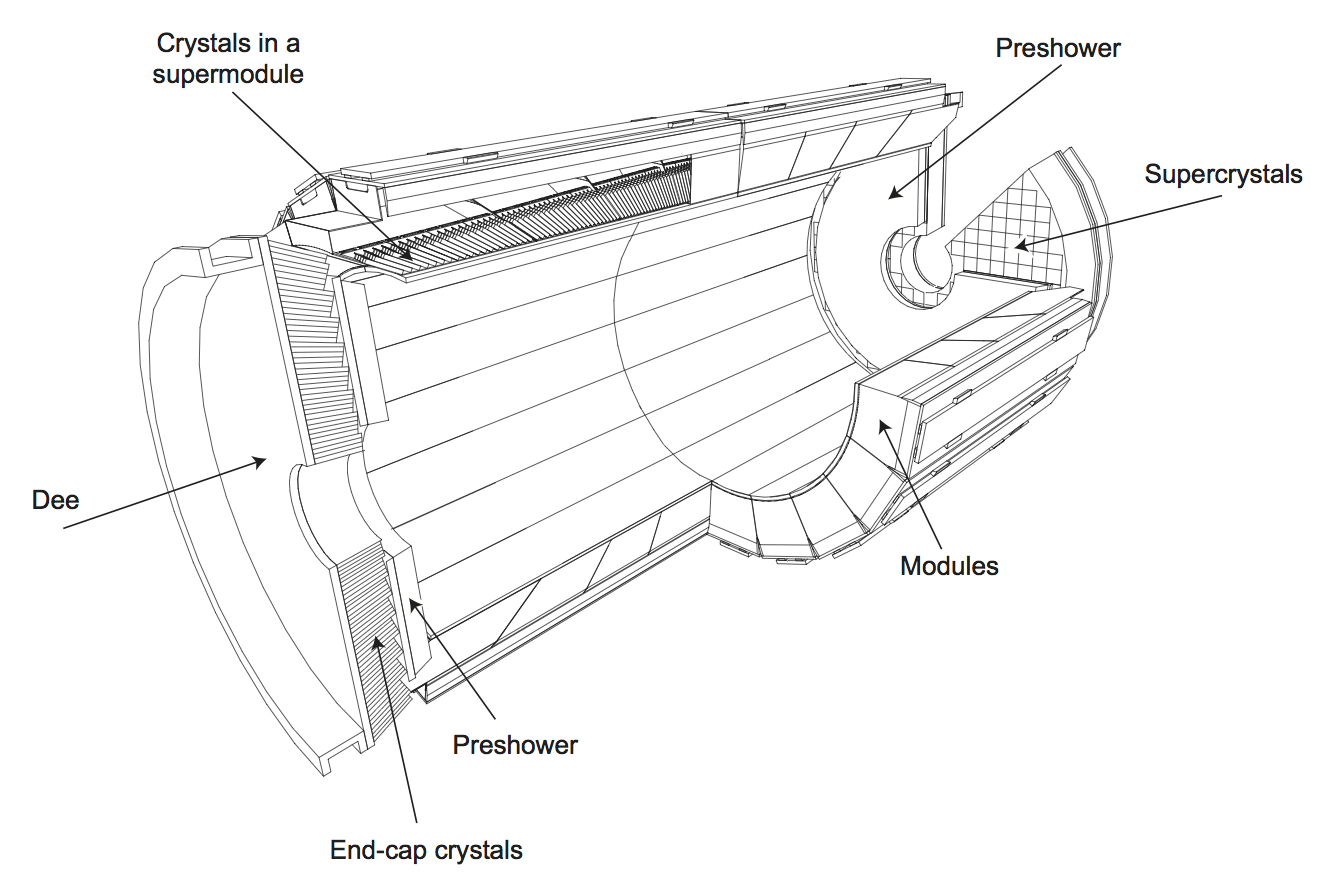
\includegraphics[width=0.8\textwidth]{Chapter02/CMS/Images/CMS_ECAL_Layout.png}
  \caption{Diagram of the ECAL layout illustrating the positions of its components. The barrel has an inner radius of $129\,\centi\meter$ and the encaps are at a distance of $315.4\,\centi\meter$ from the vertex~\cite{ARTICLE:TheCMSExperiment}.}
  \label{FIGURE:ExperimentalApparatus_CMS_ECAL_Layout}
\end{figure}
 
The energy resolution of the \gls{ECAL} can be expressed as: 

\begin{equation}
\frac{\sigma}{E} = \frac{S}{\sqrt{E}} \oplus \frac{N}{E} \oplus C
\end{equation}

Here $E$ is the energy of the incoming particle in $\GeV$, $S$ is the stochastic term, which quantifies the fluctuations in scintillation and lateral containment of the shower, $N$ the noise term, which relates to the electronics and digitisation process, and finally $C$ is a constant term that quantifies the non-uniform longitudinal response and inter-calibration errors. These parameters have been measured to be  $S=0.028\,\GeV^{1/2}$, $N=0.12\,\GeV$ and $C=0.003$ with the help of an electron beam~\cite{ARTICLE:CMSECALTestBeam} and in the absence of magnetic field.

%%%%%%%%%%%%%%%%%%%%%%%%%%%%%%%%%%%%%%%%%%%%%%%%%%%%%%%%%%%%%%%%%%%%%%%%%%%%%%%%%%%%%%%
%%% SUBSUBSECTION
%%%%%%%%%%%%%%%%%%%%%%%%%%%%%%%%%%%%%%%%%%%%%%%%%%%%%%%%%%%%%%%%%%%%%%%%%%%%%%%%%%%%
\subsubsection{Preshower detector}
\label{SUBSUBSECTION:ExperimentalApparatus_CMS_ECAL_Preshower}

% STATUS: DONE (reviewed D. Colling x1)

The \gls{CMS} Preshower is a detector located in front of each endcap covering the fiducial region of $1.653<|\eta|<2.6$. Its mission is to identify neutral pion decays, help to identify electrons against minimum ionizing particles and improve electron and photon position determination.

This detector is a sampling calorimeter composed of two layers of lead radiators each followed by silicon strip sensors. The lead layers have the function of forcing the incoming particles to initiate an electromagnetic shower. The first lead layer has $2X_0$ while the second has $1X_0$, which results in 95\% of the single incident photons starting their shower before hitting the first sensor~\cite{ARTICLE:TheCMSExperiment}. The shape of the lead layers edge matches the \gls{ECAL} crystal behind them to facilitate calculations at the \gls{L1T}.

Each silicon sensor has an active area of $61 \times 61\,\milli\meter$ and is $320\,\micro\meter$ thick. The sensors are divided into 32 strips, each $1.9\,\milli\meter$ long.  The preshower system has a total thickness of $20\,\centi\meter$ and 137000 individual read-out channels. 

%%%%%%%%%%%%%%%%%%%%%%%%%%%%%%%%%%%%%%%%%%%%%%%%%%%%%%%%%%%%%%%%%%%%%%%%%%%%%%%%%%%%%%%
%%% SUBSECTION
%%%%%%%%%%%%%%%%%%%%%%%%%%%%%%%%%%%%%%%%%%%%%%%%%%%%%%%%%%%%%%%%%%%%%%%%%%%%%%%%%%%%
\subsection{Hadronic Calorimeter}
\label{SUBSECTION:ExperimentalApparatus_CMS_HCAL}

% STATUS: DONE (reviewed D. Colling x1)

The \acrfull{HCAL} is a sampling calorimeter which is designed to measure the properties of hadron jets and indirectly neutrinos or other undiscovered particles that would result in apparent missing energy~\cite{CMSTDR:CMSHCAL}. The design of the \gls{HCAL} was strongly influenced by the choice of the magnet parameters as most of the calorimetry is inside of the magnet. A diagram of the \gls{HCAL} subsystems and their location inside \gls{CMS} can be found in figure \ref{FIGURE:ExperimentalApparatus_CMS_HCAL_Layout}.

\begin{figure}[!htb]
  \centering
  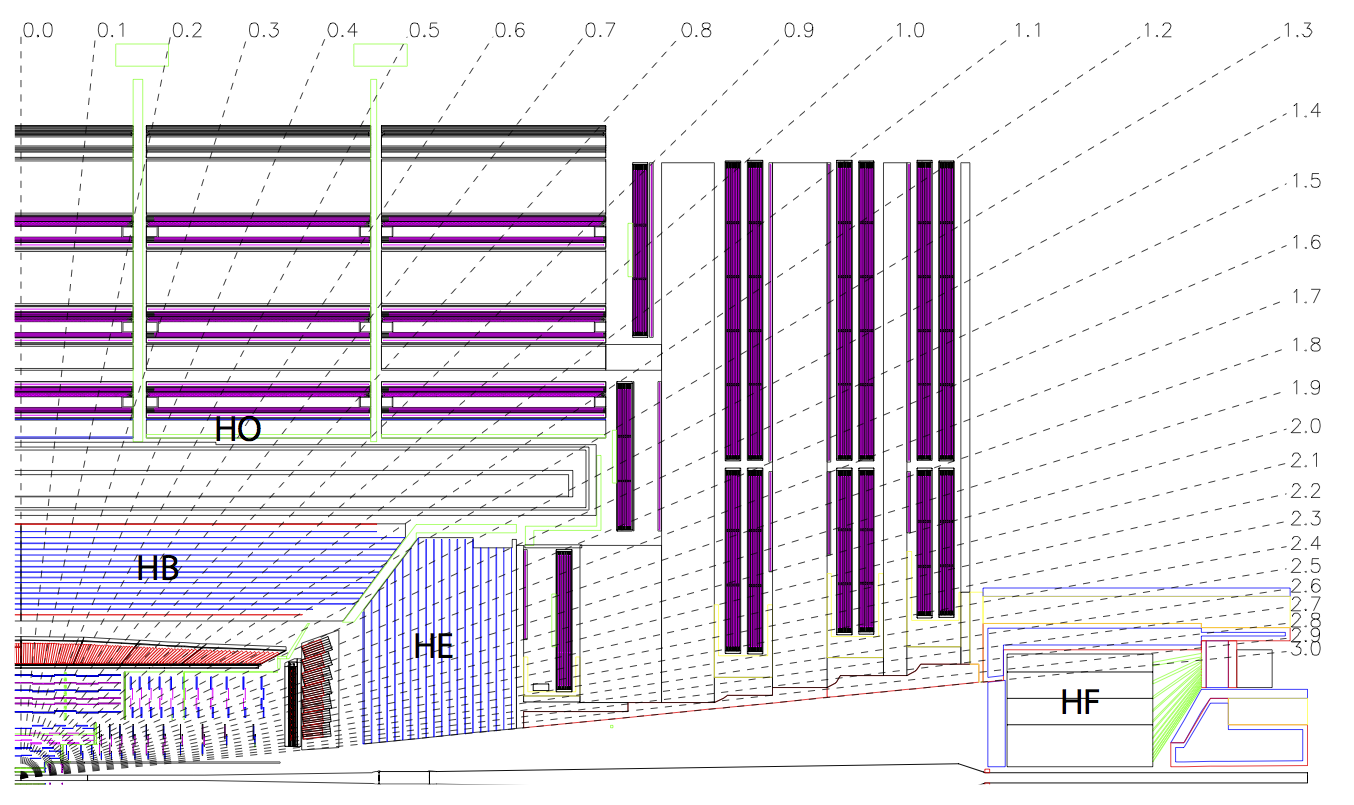
\includegraphics[width=1.0\textwidth]{Chapter02/CMS/Images/CMS_HCAL_Layout.png}
  \caption{Longitudinal view of the CMS detector highlighting the location of the \gls{HCAL} components: \gls{HB}, \gls{HE} \gls{HO} and \gls{HF}. The dashed lines show different pseudo-rapidity values. The experiment has an approximate length of  $21.6\,\metre$ long and $15\,\metre$~\cite{ARTICLE:TheCMSExperiment}.}
  \label{FIGURE:ExperimentalApparatus_CMS_HCAL_Layout}
\end{figure}

The \acrfull{HB} covers the region up to $|\eta|<1.3$ and is limited from the beam side by the \gls{ECAL} at radius $r=1.77\,\meter$ and outwards by the magnet at radius $r=2.95\,\meter$. This is a strict limitation on the amount of absorber material to be used. This detector is composed of 36 identical azimuthal wedges split in two half-barrels. They are constructed of brass absorber plates alternated with plastic scintillator. Brass has a short interaction length ($X_0=16.42\,\centi\meter$) and is non-magnetic. The detector is composed of 2304 towers with a segmentation of $\Delta\eta \times \Delta\phi = 0.087 \times 0.087$ which correspond to the same area of the $5 \times 5$ arrays of \gls{ECAL} crystals.

To improve the measurement capability, an outer calorimeter, the \acrfull{HO}, is placed outside of the magnet as a \textit{tail catcher}. It increases the effective thickness of the hadronic calorimeter by over 10 interaction lengths. This detector covers the range $|\eta|<1.26$, it is composed by an iron absorber and scintillator and is subdivided into sectors that cover 30º azimuthal angle in each of the barrel wheels. 

The \acrfull{HE} covers the range of $1.3<|\eta|<3.0$. It is composed by 2034 towers segmented in $\eta$ (14 strips) and $\phi$ (5º sectors). In the 8 innermost towers the segmentation is 10º in $\phi$, whilst the $\eta$ segmentation increases in $\eta$ from 0.09 to 0.35.

Additionally, to extend acceptance to $|\eta|<5.2$ the \gls{HF} is installed at $11.2\,\meter$ from the interaction point providing excellent hermeticity for $E_{\perp}^{miss}$ measurement. Its steel absorber is $1.65\,\meter$ deep and has quartz fibres running through it, parallel to the beam line. The energy measurement is made via Cerenkov light produced by the incoming particles inside the fibres. There are 13 towers in $\eta$ with segmentation of $\approx \Delta\eta=0.175$ except the lowest $\eta$ tower with $\approx \Delta\eta=0.1$ and highest $\eta$ tower with $\approx \Delta\eta=0.3$. The segmentation in $\phi$ is $\Delta\phi=10º$ except in the highest $\eta$ towers where $\Delta\phi=20º$. There are a total of 900 towers per \gls{HF} module. 

Similarly to the \gls{ECAL}, the energy resolution of the \gls{HCAL} was tested using a test beam of single charged pions~\cite{ARTICLE:CMSECALTestBeam}, and it was obtained that:

\begin{equation}
\frac{\sigma}{E} = \frac{94.3\%}{\sqrt{E}} \oplus 8.4\%.
\end{equation}

%%%%%%%%%%%%%%%%%%%%%%%%%%%%%%%%%%%%%%%%%%%%%%%%%%%%%%%%%%%%%%%%%%%%%%%%%%%%%%%%%%%%
%%% SUBSECTION
%%%%%%%%%%%%%%%%%%%%%%%%%%%%%%%%%%%%%%%%%%%%%%%%%%%%%%%%%%%%%%%%%%%%%%%%%%%%%%%%%%%%
\subsection{Solenoid Magnet}
\label{SUBSECTION:ExperimentalApparatus_CMS_Magnet}

%Status: DONE (reviewed D. Colling x1)

The design requirements for correct charge assignment and \pt determination for charged particles, and especially muons, drive the magnet parameters choice. For muons, unambiguous charge determination requires momentum resolution of $\Delta p/p \approx 10\%$ at $p = 1 \TeV$. These requirements are especially difficult to obtain in the forward regions but with the correct length/radius ratio can be obtained with a modestly sized solenoid magnet but with large field~\cite{CMSTDR:CMSPhysicsVol1,CMSTDR:CMSMagnet}.

The choice of the \gls{CMS} collaboration was to build a Niobium-Titanium (NbTi) superconducting solenoid magnet which has been designed to operate at fields up to $4\,\tesla$. It has a diameter of $6\,\meter$ and a length of $12.5\,\meter$ and at maximum field the stored energy reaches $2.7\,\giga\joule$. Typically, the magnet is only run at $3.8\,\tesla$ in order to maximize its lifetime. To contain such an enormous magnetic flux, a $10\,\kilo\ton$ return yoke envelopes the magnet with 5 wheels in the barrel region and 2 endcaps composed of 3 disks closing the sides~\cite{ARTICLE:TheCMSExperiment}. A summary of the most important magnet parameters can be found at table \ref{TABLE:ExperimentalApparatus_CMSMagnetParameters}.

\begin{table}[!htb]
  \centering
  \begin{tabular}{|l|c|}
  \hline
  Parameter & Value \\
  \hline\hline
  Field           & 4 T \\
  Inner Bore      & 5.9 m \\
  Length          & 12.9 m \\
  Number of turns & 2168 \\
  Current         & 19.5 kA \\
  Stored Energy   & 2.7 GJ \\
  Hoop Stress     & 64 atm \\
  \hline
  \end{tabular}
  \caption[Parameters of the CMS superconducting solenoid]{Parameters of the CMS superconducting solenoid}
  \label{TABLE:ExperimentalApparatus_CMSMagnetParameters}
\end{table}


%%%%%%%%%%%%%%%%%%%%%%%%%%%%%%%%%%%%%%%%%%%%%%%%%%%%%%%%%%%%%%%%%%%%%%%%%%%%%%%%%%%%
%%% SUBSECTION
%%%%%%%%%%%%%%%%%%%%%%%%%%%%%%%%%%%%%%%%%%%%%%%%%%%%%%%%%%%%%%%%%%%%%%%%%%%%%%%%%%%%
\subsection{Muon System}
\label{SUBSECTION:ExperimentalApparatus_CMS_Moun}

%Status: DONE (reviewed D. Colling x1)

The muon detection is an important part of the mission of \gls{CMS}~\cite{CMSTDR:CMSMuonSystem}. Muons are fairly easy to detect when compared with other elementary particles and are only rarely produced in proton-proton collisions. Taking the example of a \gls{SM} Higgs boson with $m_H=125\,\GeV$, while the decay mode involving a pair of Z bosons is fairly unlikely, only happening $\approx 2.64\%$ of the times~\cite{ARTICLE:PDG2014}, the Z bosons can decay into 4 muons. This decay, while rare, does not have significant backgrounds making it a ``golden channel'' for discovery, which indeed has proven the case~\cite{ARTICLE:CMSHiggsObservation}. Many other models, like \gls{SUSY}, use muon final states in their searches for exactly the same reason. The \gls{CMS} muon system is composed of 3 types of gaseous detectors depending on the location and momentum reconstruction needs. A diagram of the disposition of this system inside \gls{CMS} can be found on figure \ref{FIGURE:ExperimentalApparatus_CMS_Muon_Layout}.

\begin{figure}[!htb]
  \centering
  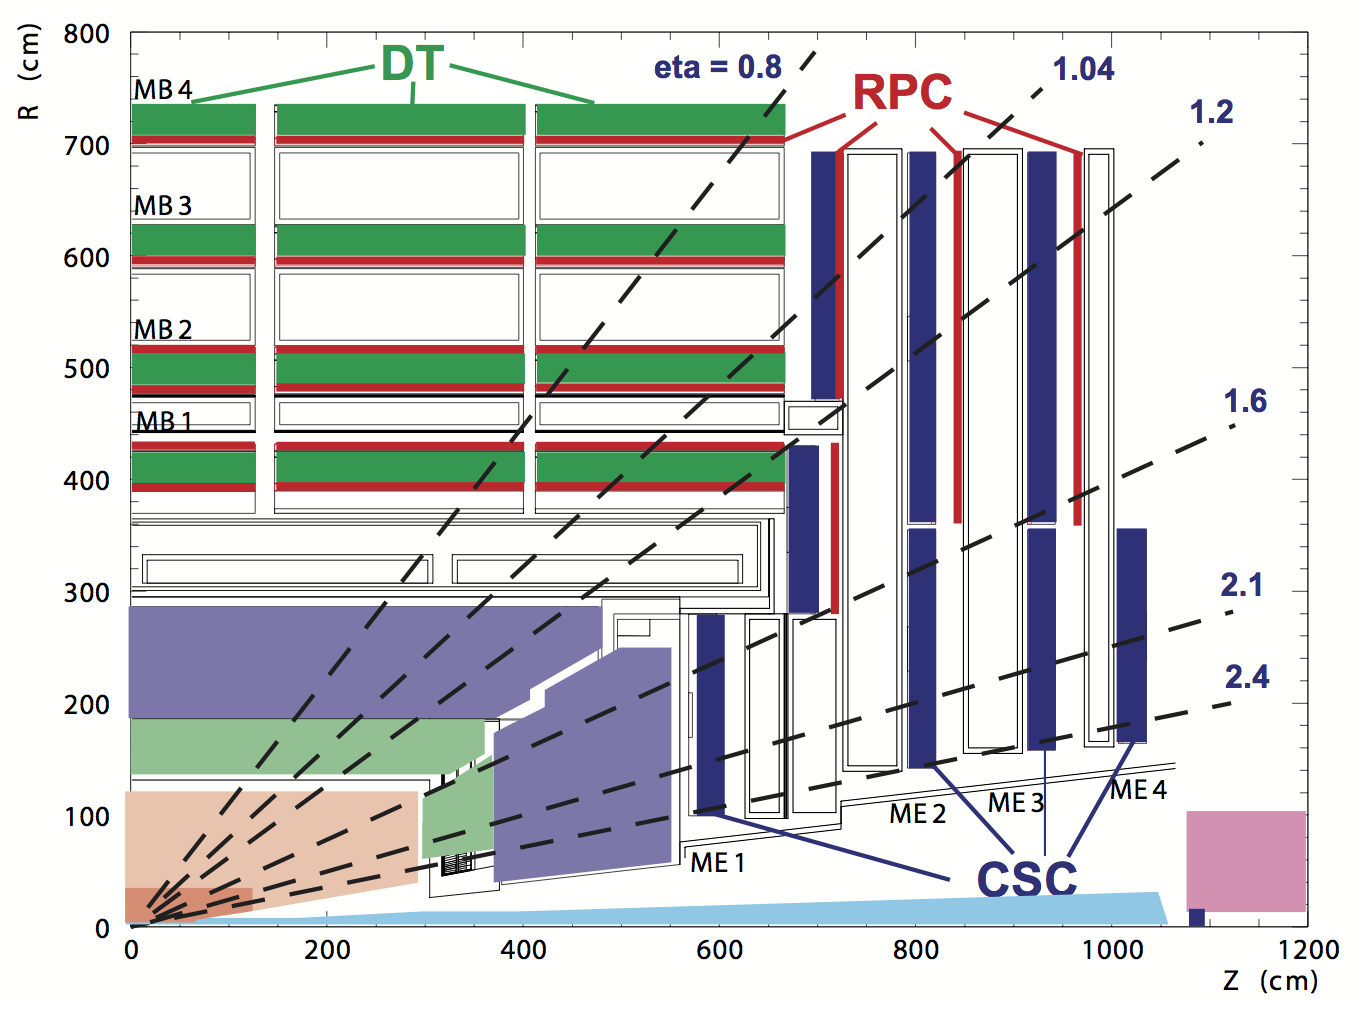
\includegraphics{Chapter02/CMS/Images/CMS_Muon_Layout.png}
  \caption{Diagram of the \gls{CMS} muon systems. The location of each muon chamber for each subsystem is shown: \gls{DT}, \gls{CSC} and \gls{RPC}~\cite{CMSTDR:CMSPhysicsVol1}.}
  \label{FIGURE:ExperimentalApparatus_CMS_Muon_Layout}
\end{figure}

In the barrel and up to $|\eta|<1.2$, \acrfull{DT} are used, since the neutron background is small and the field is constant. This system is composed of 250 chambers and is arranged in 4 concentric cylindrical layers which are installed inside of the return yoke. These chambers have a total of 172000 wires with a length of $2.4\,\meter$ which are housed inside of tubes filled with a mixture of argon and carbon-dioxide. Each of the barrel wheels is split into 12 sectors covering 30º azimuthal angle. The maximum gas ionization drift is $2.0\,\centi\meter$ and results in a single point resolution of $\approx 200\,\micro\meter$ per wire. For each station and each measured muon, the $\phi$ resolution is better than $200\,\micro\meter$ and the direction resolution is $\approx 1\,\milli\radian$.

In the endcaps, \gls{CSC} are used in the region between $2.4>|\eta|>0.9$. Here, muon and background rates are high and the magnetic field is not uniform. This system has fast response and is radiation resistant. It is composed of 468 chambers arranged in 4 stations per side. Each chamber is trapezoidal in shape and made of 6 gas gaps and covers either 10º or 20º in $\phi$. Each gap contains a plane of cathode strips and a plane of anode wires. For each chamber the spatial resolution is of the order of $200\,\micro\meter$ and the angular resolution is $\approx 10\,\milli\radian$ in $\phi$.

Finally the \gls{RPC} covers the $|\eta|<1.6$ range. This system overlaps with the 2 other muon systems. It is very fast with an ionization event being much faster than the bunch crossing time. This fast response allows, in conjunction with a dedicated trigger system, the correct bunch crossing associated with the detection of a muon to be selected. In the barrel, there are 480 rectangular chambers arranged in 4 stations with 6 \gls{RPC} layers (2 layers are present in the 2 stations closest to the beam pipe). In the endcaps there are 3 \gls{RPC} disk shaped stations on each side, which are composed by trapezoidally shaped detectors.

The combined muon system offline momentum resolution is of the order of 9\% for small values of $\eta$ and $p$ and for transverse momenta of up to $200\,\GeV$. At higher energies of around $1\,\TeV$ the standalone momentum resolution is in the range of 15-40\% depending on $|\eta|$. These values are limited by the muon multiple-scattering before arriving to the muon system. If we combine the tracker information into a global fit the resolution for lower \pt tracks improves an order of magnitude while at higher momenta (around $1\,\TeV$) it is about 5\%, which is well inside the \gls{CMS} design requirements.

%%%%%%%%%%%%%%%%%%%%%%%%%%%%%%%%%%%%%%%%%%%%%%%%%%%%%%%%%%%%%%%%%%%%%%%%%%%%%%%%%%%%%%%
%%% SUBSECTION
%%%%%%%%%%%%%%%%%%%%%%%%%%%%%%%%%%%%%%%%%%%%%%%%%%%%%%%%%%%%%%%%%%%%%%%%%%%%%%%%%%%%
\subsection{Data Acquisition System}
\label{SUBSECTION:ExperimentalApparatus_CMS_DAQ}

%Status: DONE (reviewed D. Colling x1)

The \gls{CMS} \gls{DAQ} system is designed to process, analyse and ultimately store the information collected by the detector~\cite{CMSTDR:CMSTridasTDRVol2}. The \gls{LHC} produces bunch crossings at a rate of up to $40\,\mega\hertz$ but we are only capable of storing between $10^2-10^3$ events per second. At design luminosity, each bunch crossing will have an average of over 20 simultaneous collisions and produce a zero-suppressed data payload of around $1\,\mega\byte$. A first level of trigger was developed in order to reduce the event rate to a maximum of $100 \kilo\hertz$ and only the selected events are fully retrieve from the detector event buffers. Even with this event suppression the \gls{DAQ} has to retrieve and move $\approx 100\, \giga\byte/\second$ from the detector to the surface. This data comes from approximately 650 data sources and has to be merged into a single event package. The information is then passed to a computer farm where software filters serve as a second level of trigger. In this system the event rate is further reduced by a factor of up to 1000 making the output rate compatible with what can be saved into permanent storage. A diagram of this system can be found on figure \ref{FIGURE:ExperimentalApparatus_CMS_DAQ_Diagram}.

\begin{figure}[!htb]
  \centering
  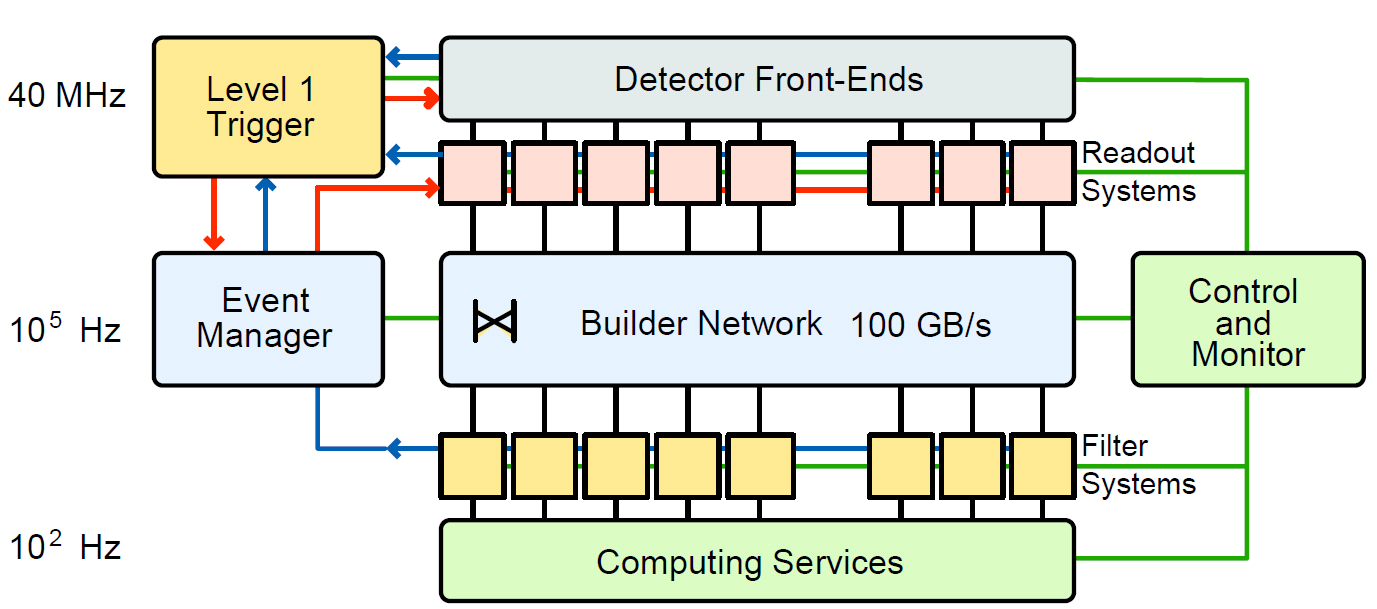
\includegraphics[width=0.80\textwidth]{Chapter02/CMS/Images/CMS_DAQ_Diagram.png}
  \caption{Diagram of the \gls{CMS} \gls{DAQ} system. Data flow is showed as the lines connecting each electronics or computing units~\cite{ARTICLE:TheCMSExperiment}.}
  \label{FIGURE:ExperimentalApparatus_CMS_DAQ_Diagram}
\end{figure}

%%%%%%%%%%%%%%%%%%%%%%%%%%%%%%%%%%%%%%%%%%%%%%%%%%%%%%%%%%%%%%%%%%%%%%%%%%%%%%%%%%%%%%%
%%% SUBSECTION
%%%%%%%%%%%%%%%%%%%%%%%%%%%%%%%%%%%%%%%%%%%%%%%%%%%%%%%%%%%%%%%%%%%%%%%%%%%%%%%%%%%%
\subsection{Trigger System}
\label{SUBSECTION:ExperimentalApparatus_CMS_Trigger}

%Status: DONE (reviewed D. Colling x1)

The \gls{CMS} trigger system is responsible for selecting which collisions are recorded in real-time. We can only save $\mathcal{O}(10^2-10^3)$ events per second with the current systems. This implies that the trigger system needs to obtain a data reduction of a factor of $\mathcal{O}(10^6-10^7)$. This is achieved with a two level trigger system, the first is a dedicated hardware system named \acrfull{L1T}~\cite{CMSTDR:CMSTridasTDRVol1} and the second is a commercial computer farm running dedicated software called the \gls{HLT}~\cite{CMSTDR:CMSTridasTDRVol2}.

Initially, all data is stored for 128 bunch crossings which corresponds to $3.2\,\micro\second$. This is the time we have to make a first decision to keep or discard an event. This is the task of the \gls{L1T} which has the target to reduced the data to a maximum rate of $100\,\kilo\hertz$. There isn't enough time to get all the information from the detector, so only a coarse version of the calorimetry and muon systems data, and some correlation between them is accessed. With this information the \gls{L1T} produces a set of particle candidates and energy sums over which custom, user-defined algorithms can be used to filter events. A diagram of the \gls{L1T} trigger components and the data flow across the system is present on figure \ref{FIGURE:ExperimentalApparatus_CMS_L1T_Layout}.

\begin{figure}[!htb]
  \centering
  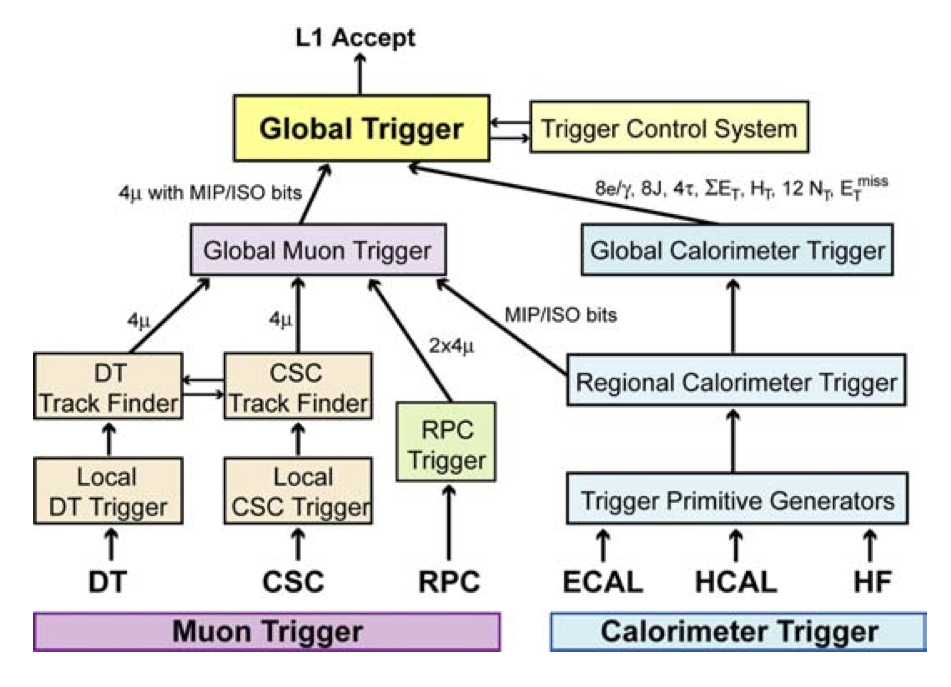
\includegraphics[width=0.80\textwidth]{Chapter02/CMS/Images/CMS_L1T_Layout.png}
  \caption{Diagram of the \gls{L1T} system. The arrows indicate data flow and the number of particle candidates at each step is indicate~\cite{ARTICLE:TheCMSExperiment}.}
  \label{FIGURE:ExperimentalApparatus_CMS_L1T_Layout}
\end{figure}

The \gls{HLT} receives events accepted by the \gls{L1T} and needs to perform further event reduction of 
$\mathcal{O}(10^{3}-10^{2})$ to a final output rate of $\mathcal{O}(10^{2}-10^{3})\,\hertz$. This system is composed of standard computing hardware in the form of a computing farm with $\approx 15\,\kilo$ \glspl{CPU}. This system, using the additional latency created by the \gls{L1T} event selection, is able to make use of the complete detector information including the tracker data. More sophisticated and precise algorithms are therefore possible which can be tailored to select any desired physical final state. An \gls{HLT} path is defined by the sequence of requirements for an event to be accepted, starting with the selection of the seeding \gls{L1T} algorithms followed by \gls{HLT} object requirements.

Event selection algorithms at both the \gls{L1T} and \gls{HLT} are frequently updated during data taking. The selection thresholds may be tuned in order to control the rate with the changes of \gls{LHC} luminosity. Novel methods or strategies to identify particles more efficiently can be implemented, like \gls{PU} subtraction or new calibrations. Analysis groups may also show interest in recording new event final states for which new selection criteria may be developed. The set of algorithms used for data taking is normally referred to as the \textit{trigger menu}. 

After events pass both levels of the trigger they are recorded into permanent storage. During 2012-13 operation, two output streams were saved. The \textit{prompt data stream}, with a rate of approximately $300\,\hertz$, was composed of high priority trigger paths which were immediately reconstructed. And the \textit{parked data stream}, with an average rate of $600\,\hertz$, was stored without reconstruction. These data waited until computing resources were free to go through reconstruction~\cite{ARTICLE:CMSDataParking}. This process was finalised a few months after the \gls{LHC} Run I was finished.

Even with such measures to reduce the data to be stored, each \gls{LHC} experiment records several petabytes of data every year in addition to similarly sized amounts of simulated events.

%%%%%%%%%%%%%%%%%%%%%%%%%%%%%%%%%%%%%%%%%%%%%%%%%%%%%%%%%%%%%%%%%%%%%%%%%%%%%%%%%%%%%%%
%%% SUBSECTION
%%%%%%%%%%%%%%%%%%%%%%%%%%%%%%%%%%%%%%%%%%%%%%%%%%%%%%%%%%%%%%%%%%%%%%%%%%%%%%%%%%%%
\subsection{Computing}
\label{SUBSECTION:ExperimentalApparatus_CMS_Computing}

%Status: DONE (reviewed D. Colling x1)

The quantity of data produced by the \gls{LHC} and the necessary processing capability is so big that it would be difficult to have all computing resources in a single place. For this reason a tiered system was developed, where all participating computing sites are connected and have specific roles and responsibilities in the data taking, processing and storing. This global computing system is known as the Grid~\cite{CMSTDR:CMSComputing}.

The \gls{CERN} Data Centre is the Tier 0 of this network, all data produced by the \gls{LHC} experiments is handled by this facility. Only about 20\% of the total capacity of the Grid is hosted here, but the \gls{CERN} Tier 0 has the very important mission of safe keeping all the raw data produced by the experiments. It also has the task of doing the first pass of event reconstruction, which is the process identifying meaningful physics objects in data.

There are 7 \gls{CMS} Tier 1 computer centres around the world. They are responsible to store a proportional amount of raw and reconstructed data for safe keeping. If any reprocessing of the data is needed, these centres are responsible for this task and for storing the resulting output as well. 

Local research centres like universities of scientific laboratories are normally at the Tier 2 level. These centres have the responsibility of handling a proportional share of simulated data production and reconstruction. Currently there are over 150 Tier 2 centres around the world. All physics analysis happen at this level.

Individual computers or local clusters without any formal engagement with the Grid structure, are considered to be the Tier 3 level of the Grid. 

%%%%%%%%%%%%%%%%%%%%%%%%%%%%%%%%%%%%%%%%%%%%%%%%%%%%%%%%%%%%%%%%%%%%%%%%%%%%%%%%%%%%%%%
%%% SUBSECTION
%%%%%%%%%%%%%%%%%%%%%%%%%%%%%%%%%%%%%%%%%%%%%%%%%%%%%%%%%%%%%%%%%%%%%%%%%%%%%%%%%%%%
\subsection{Level 1 Trigger: Stage I Upgrade}
\label{SUBSECTION:ExperimentalApparatus_CMS_L1TStage1}

%Status: DONE (reviewed D. Colling x1)

An extensive upgrade program for the \gls{L1T} electronics was planed and is being executed in order to cope with the increase of luminosity and pile-up predicted for Run II~\cite{CMSTDR:CMSL1Upgrade,CMSTDR:CMSUpgradeTDR}. The center-of-mass energy has almost doubled from $8\,\TeV$ to $13\,\TeV$, instantaneous luminosity will also increase, as will the average pile-up. Also, the bunch separation has changed from $50\,\nano\second$ to $25\,\nano\second$ making out-of-time pile-up a significant problem. 

To ensure physics performance during 2015 and beyond, only a partial upgrade was executed for the 2015 run which is known as the \textit{Stage-1} upgrade. The main feature of this upgrade program is the replacement of the existing \gls{GCT}. Two key enhancements were possible: 

\begin{itemize}
  \item Event-by-event pile-up energy subtraction for jet reconstruction, $e/\gamma$ isolation, $\tau$ isolation.
  \item Smaller feature size $\tau$ candidates, which have significantly better energy estimation and background rejection.
\end{itemize}

The intermediate system will have significantly better performance than the now legacy system. The full 2016 calorimeter trigger system will additionally provide finer granularity which will lead to increased position and energy resolution. 
